\title{Eigen values, Taylor Series, and Stability Review}
\date{}

\documentclass[12pt]{article}
\usepackage{graphicx}
\usepackage{float}
\usepackage{hyperref}
\usepackage{cite}
\usepackage{subfig}
\usepackage{enumitem}
\usepackage{amsmath}
\usepackage{listings}
%\usepackage{fullpage}
%\bibliographystyle{science}
\bibliographystyle{plain}

\lstdefinelanguage{Maxima}{
  keywords={addrow,addcol,zeromatrix,ident,augcoefmatrix,ratsubst,diff,ev,tex,%
    with_stdout,nouns,express,depends,load,submatrix,div,grad,curl,%
    rootscontract,solve,part,assume,sqrt,integrate,abs,inf,exp},
  sensitive=true,
  comment=[n][\itshape]{/*}{*/}
}

\newif\ifanswers
%\answerstrue % comment out to hide answers

\begin{document}
\maketitle

\section{Linear stability analysis}
This review sheet has been adapted from a set of notes written by Gordon Brown in 1990, titled ``Stability Analysis of Continuous Single-Species Population Models''.

A model of population growth such as:
\begin{equation}
\frac{dN}{dt} = F(N)
\end{equation}
will have equilibrium point $N^{*}$ when:
\begin{equation}
\frac{dN}{dt} = 0
\end{equation}

Assuming that $N^{*}$ is found, one might wish to determine its stability - i.e. if N is perturbed away from $N^{*}$, will it return to $N^{*}$ or move to some other value? Linear stability analysis can help answer this question, provided that the perturbation is ``small'' (unfortunately, what constitutes a ``small'' perturbation depends on the equation being analyzed). This handout will attempt to illustrate some of the logic behind linear stability analysis, and is designed to complement Dr. Tilman's discussion. Let:

\begin{equation}
N = N^{*} + a(t)
\end{equation}

therefore:
\begin{equation}
a(t) = N - N^{*}
\end{equation}

Linear stability analysis determines the fate of the function $a(t)$, which indicates the magnitude of the deviation from equilibrium, as t approaches infinity. If $a(t) \rightarrow 0$, then $N$ returns to $N^{*}$. To examine the dynamics of $a(t)$, we find its derivative:

\begin{equation}
\begin{split}
\frac{d}{dt}(a(t)) = \frac{d}{dt}(N-N^{*})\\
= \frac{dN}{dt} \mathrm{(since N^{*} is a constant)}
\end{split}
\end{equation}

An expression for $\frac{dN}{dt}$ in terms of $a(t)$ and $t$ is now needed. Recall that $\frac{dN}{dt} = F(N)$, and that we are examining values of N which are close to $N^{*}$. In order to derive our function of $a(t)$ at $t$, we will expand $F(N)$ about the value $N^{*}$ using a Taylor Series approximation. The formula for the Taylor Series is:

\begin{equation}
f(x) = f(a) + \frac{df}{dx}|_{x=a}(x-a) + \frac{\frac{d^{2}f}{dx^{2}}}{2!}|_{x=a}(x-a)^{2} + \frac{\frac{d^{3}f}{dx^{3}}}{3!}|_{x=a}(x-a)^{3} + ...
\end{equation}

where $a$ is a value for $x$. When applied to our case, we get:
\begin{equation}
F(N) = F(N)|_{N^{*}} + \frac{dF}{dN}|_{N^{*}}(N-N^{*}) + \frac{\frac{d^{2}F}{dN^{2}}}{2!}|_{N^{*}}(N-N^{*})^{2} + \frac{\frac{d^{3}F}{dN^{3}}}{3!}|_{N^{*}}(N-N^{*})^{3} + ...
\end{equation}

We only use the first two terms of this series to yield a linear equation which approximates $F(N)$ (this is why this procedure is called linear stability analysis).

\begin{equation}
F(N) \approx F(N)|_{N^{*}} + \frac{dF}{dN}|_{N^{*}}(N-N^{*})
\end{equation}

However, since $F(N^{*}) = 0$, this simplifies further to $F(N) \approx \frac{dF}{dN}|_{N^{*}}(N-N^{*})$.

Recall that $\frac{d}{dt}(a(t)) = \frac{dN}{dt} = F(N)$, and $a(t) = N - N^{*}$. Substituting these relationships into the linear approximation for $F(N)$ yields:

\begin{equation}
\frac{d}{dt}(a(t)) = \frac{d}{dN}(F(N))|_{N^{*}}a(t)
\end{equation}

If we let $\frac{d}{dN}(F(N))|_{N^{*}} = \lambda$, then we simply get:

\begin{equation}
\frac{d}{dt}(a(t)) = \lambda a(t)
\end{equation}

We now have our differential equation in terms of $a(t)$ and $t$, and can use it to determine the dynamics of $a(t)$, the deviation of population size from its equilibrium value. First, we must solve for $a(t)$:

\begin{equation}
\begin{split}
(\frac{1}{a(t)})d(a(t)) = \lambda dt\\
\int (\frac{1}{a(t)})d(a(t)) = \int \lambda dt\\
\log(a(t)) + K_{1} = \lambda t + K_{2}\\
\end{split}
\end{equation}

let $K = K_{2} - K_{1}$

\begin{equation}
\begin{split}
\log(a(t)) = \lambda t + K\\
e^{\log(a(t))} = e^{\lambda t + K}\\
\end{split}
\end{equation}

let $e^{K} = K'$

\begin{equation}
a(t) = K' e^{\lambda t}\\
\end{equation}

let $t=0$ to find the initial perturbation

\begin{equation}
\begin{split}
a(0) = K' e^{\lambda 0}\\
K' = a(0)\\
a(t) = a(0) e^{\lambda t}
\end{split}
\end{equation}

Here is our equation to determine the dynamics of the perturbation with time. Obviously, if $c<0$, then the perturbation decays away exponentially with time, and the population returns to its equilibrium value; the equilibrium is therefore stable. If $c>0$, then the perturbation grows exponentially with time; the equation is unstable. If $c=0$, then the equilibrium is neutrally stable; the perturbation does not grow or shrink with time (at least, according to our linearized system). Remember that:

\begin{equation}
c = \frac{d}{dN}(F(N))|_{N^{*}}
\end{equation}

Therefore the sign of $\frac{d}{dN}(F(N))$ at the equilibrium point determines the stability of that equilibrium.

\section{A Worked Example}

Consider the standard logistic growth model $F(N)=\frac{dN}{dt}=rN(1-\frac{N}{K})=rN-\frac{rN^{2}}{K}$. This model has two equilibria, at $N=0$ and $N=K$. Differentiating by $N$, we get:

\begin{equation}
\begin{split}
\frac{d}{dN}(F(N)) = r - \frac{2rN}{K}
\end{split}
\end{equation}

For equilibrium $N=0$, we solve $\frac{d}{dN}(F(N)) = r - 0 = r = \lambda$. Thus, provided that $r$ is positive, we expect deviations from this equilibrium to grow roughly following $e^{r}$, and the point is thus unstable (leftmost blue line in figure).

For equilibrium $N=K$, we solve $\frac{d}{dN}(F(N)) = r - \frac{2rK}{K} = r - 2r = -r = \lambda$. Thus, provided that $r$ is positive, we expect deviations from equilibrium to shrink back to $K$ roughly following $e^{-r}$ (right red and blue lines in the figure).
 
Since all known organisms have a positive growth rate in an unlimited environment, this analysis indicates that the equilibrium at zero is unstable $(\lambda>0)$, and that the equilibrium at $K$ is locally stable $(\lambda<0)$. The equilibrium at $K$ is also globally stable, but that's another story.

\begin{figure}[H]
  \centering
  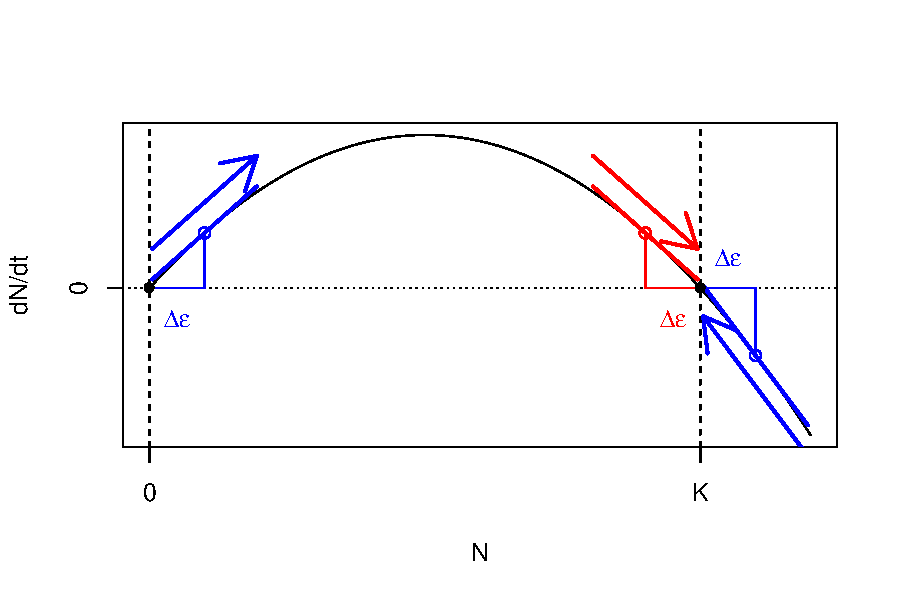
\includegraphics[width=0.75\textwidth, page=1]{figures/Eigen_Linear}
  \caption{Linearized stability analysis. Dynamics following small perturbations around equilibrium $\Delta \epsilon$ can be estimated using a first-order Taylor expansion. Thick lines show these derivatives, and arrows show the resulting directions of flow on either side of the equilibrium.}
\end{figure}


\end{document}